\section{数据爬取}
\subsection{爬取对象}
本报告选取共青团中央的官方微博如图 \ref{fig:gqtzy},爬取时间范围为2019年1月1日到2023年7月16日。

\begin{figure}[H]
    \centering
    
\includegraphics[width=12cm]{figure/gqtzy.jpg}
    \caption{共青团中央官方微博} \label{fig:gqtzy}
\end{figure}

\subsection{爬虫实现}
本报告数据爬取使用Github基于weibo.com的新版API构建的爬虫项目,项目地址为:https://github.com/nghuyong/WeiboSpider,项目主页如图\ref{fig:weibospider}所示。主要使用该项目下的tweet.py基于用户id进行爬虫,项目具体使用可参照其README文件。
\begin{figure}[H]
    \centering
    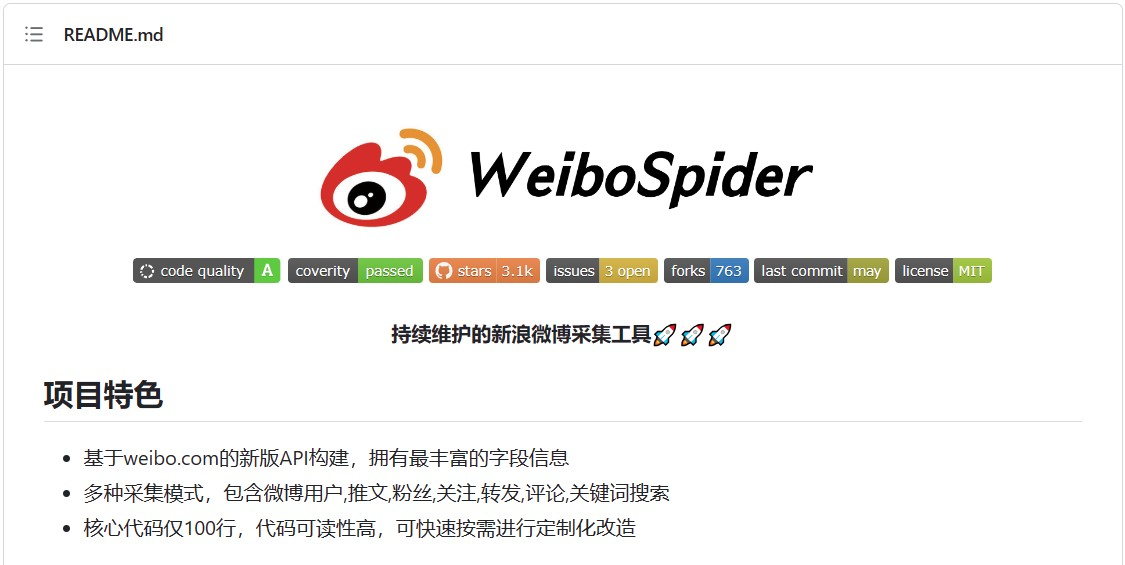
\includegraphics[width=13cm]{figure/weibospider.jpg}
    \caption{项目主页示例} \label{fig:weibospider}
\end{figure}\
该项目将爬取数据解析后存储为json格式,其单条数据示例如下所示。
\begin{python}
{
    "_id": "4762810834227120",
    "mblogid": "LqlZNhJFm",
    "created_at": "2022-04-27 10:20:54",
    "geo": null,
    "ip_location": null,
    "reposts_count": 1890,
    "comments_count": 1924,
    "attitudes_count": 12167,
    "source": "三星Galaxy S22 Ultra",
    "content": "生于乱世纵横四海,义之所在不计生死,孤勇者陈恭一生当如是。#风起陇西今日开播# #风起陇西#  今晚,恭候你!",
    "pic_urls": [],
    "pic_num": 0,
    "isLongText": false,
    "user": {
        "_id": "1087770692",
        "avatar_hd": "https://tvax1.sinaimg.cn/crop.0.0.1080.1080.1024/40d61044ly8gbhxwgy419j20u00u0goc.jpg?KID=imgbed,tva&Expires=1682768013&ssig=r1QurGoc2L",
        "nick_name": "陈坤",
        "verified": true,
        "mbrank": 7,
        "mbtype": 12,
        "verified_type": 0
    },
    "video": "http://f.video.weibocdn.com/o0/CmQEWK1ylx07VAm0nrxe01041200YDIc0E010.mp4?label=mp4_720p&template=1280x720.25.0&ori=0&ps=1CwnkDw1GXwCQx&Expires=1682760813&ssig=26udcPSXFJ&KID=unistore,video",
    "url": "https://weibo.com/1087770692/LqlZNhJFm",
    "crawl_time": 1682757213
}
\end{python}

\subsection{数据采集结果}
本报告共采集到共青团中央从2019年1月1日至2023年7月16日发微数据25244条,采集结果如图\ref{fig:outputjson}所示。
\begin{figure}[H]
    \centering
    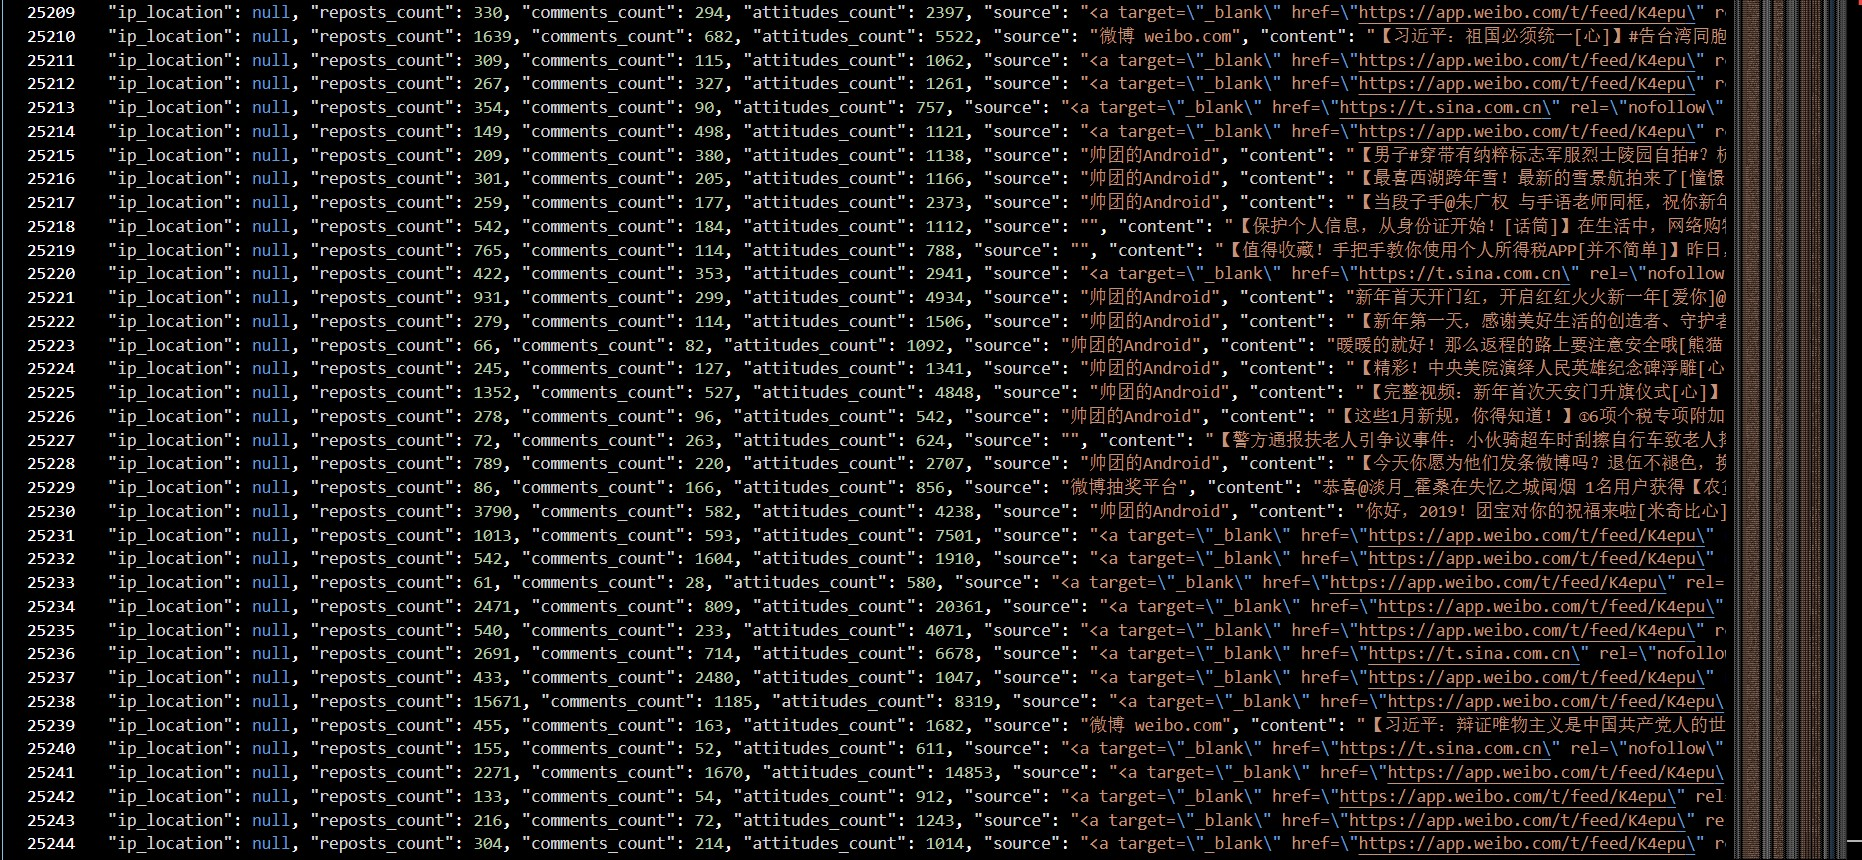
\includegraphics[width=13cm]{figure/output_1.jpg}
    \caption{数据采集结果} \label{fig:outputjson}
\end{figure}
